\subsubsection{Sesto periodo (2024/02/13 - 2024/03/06)}
\subsubsubsection{Planning}
\subsubsubsubsection*{Attività pianificate}
All'inizio del periodo ad ogni membro del gruppo sono stati assegnati ruoli specifici, di seguito riportati:
\begin{table}[H]
\centering
\begin{tabular}{|c|c|c|}
\hline
\textbf{Membro} & \textbf{Ruolo} \\
\hline
Samuele V. & Analista \\
\hline
Michele Z. & Responsabile \\
\hline
Leonardo B. & Amministratore \\
\hline
Riccardo Z. & Analista \\
\hline
Filippo T. & Verificatore \\
\hline
Davide B. & Analista \\
\hline
\end{tabular}
\caption{Ruoli assunti per ciascun membro del team all'inizio del periodo}
\end{table}

Gli obiettivi posti per lo $\textit{sprint}_G$ sono stati i seguenti:
\begin{itemize}
    \item Ultimare gli ultimi \emph{UC} e il documento di \emph{Analisi dei Requisiti};
    \item Iniziare a redigere il glossario tecnico e implementare un'insieme di automazioni utili alla sua costruzione automatica;
    \item Riprendere lo sviluppo del \emph{PoC}.
\end{itemize}


\subsubsubsubsection*{Preventivo}
\begin{table}[H]
    \centering
\begin{spreadtab}{{tabular}{|c|c|c|c|c|c|c|c|}}
    \hline
    @\textbf{Membro} & @\textbf{Re} & @\textbf{Amm} & @\textbf{An} & @\textbf{Progr} & @\textbf{Proge} & @\textbf{Ve} & @\textbf{Totale} \\
    \hline
    @ Samuele V.   & 0          & 0          & 8         & 0          & 0     & 0     & sum(b2:g2) \\
    @ Leonardo B.  & 0         & 3          & 0        & 2.5        & 0     & 0    & sum(b3:g3) \\
    @ Riccardo Z.  & 0          & 0          & 8.5          & 0          & 0     & 0   & sum(b4:g4) \\
    @ Davide B.    & 0          & 0          & 8       & 1.5       & 0     & 0     & sum(b5:g5) \\
    @ Michele Z.   & 5          & 0          & 0         & 0          & 0     & 0     & sum(b6:g6) \\
    @ Filippo T.   & 0          & 0          & 0         & 0          & 0     & 4.5     & sum(b7:g7) \\
    \hline
    @\textbf{Ore totali} & sum(b2:b7) & sum(c2:c7) & sum(d2:d7) & sum(e2:e7) & sum(f2:f7) & sum(g2:g7) &  sum(b8:g8)\\
    \hline
    @\textbf{Costo totale} & 30*b8 & 20*c8 & 25*d8 & 15*e8 & 25*f8 & 15*g8 & sum(b9:g9)\\
    \hline
\end{spreadtab}
    \caption{Preventivo orario ed economico parziale per il sesto periodo, in base al ruolo}
    \label{tab:prev_rtb}
    \vspace{5mm}
    \textbf{Legenda:} \textit{Re} = Responsabile, \textit{Amm} = Amministratore, \textit{An} = Analista, \textit{Progr} = Programmatore, \textit{Proge} = Progettista, \textit{Ve} = Verificatore
\end{table}

\newpage

\begin{figure}[H]
  \centering
  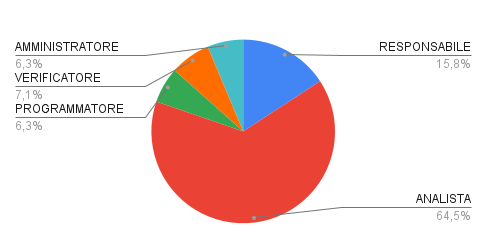
\includegraphics[width=0.6\linewidth]{grafici/6_periodo_torta.png}
  \caption{Ripartizione dei costi per ruolo nel $6^\circ$ periodo}
        \vspace{10mm}
  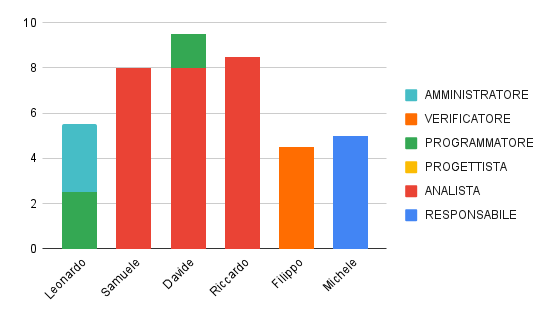
\includegraphics[width=0.7\linewidth]{grafici/6_periodo_istogramma.png}
  \caption{Ore preventivate per ciascuna persona nel $6^\circ$ periodo}
\end{figure}

\subsubsubsection{Review}
\subsubsubsubsection*{Attività svolte}
\begin{itemize}
    \item Il gruppo ritiene di aver raggiunto un livello soddisfacente per poter presentare il documento \emph{Analisi dei Requisiti} ad Imola informatica e poter dedicarsi maggiormente allo sviluppo del \emph{PoC};
    \item E' stato effettuato un incontro con il proponente il 28/2/2024 per risolvere qualche dubbio e per fare il punto della situazione. In particolare:
    \begin{itemize}
        \item Aggiornamento sullo stato dei lavori.
        \item Fissata una ipotetica data di consegna del \emph{PoC}.
        \item $\textit{Feedback}_G$ sull'attuale versione dell'\emph{Analisi dei Requisiti} e aggiornamento  sulle $\textit{tecnologie}_G$ da usare, in particolare \emph{NestJs} per il Back-End.
        \item Supporto sulla scelta della quantità di ristoranti amministrabili da un admin.
        
    \end{itemize}
\end{itemize}
\subsubsubsubsection*{Consuntivo}
\begin{table}[H]
    \centering
\begin{spreadtab}{{tabular}{|c|c|c|c|c|c|c|c|}}
    \hline
    @\textbf{Membro} & @\textbf{Re} & @\textbf{Amm} & @\textbf{An} & @\textbf{Progr} & @\textbf{Proge} & @\textbf{Ve} & @\textbf{Totale} \\
    \hline
    @ Samuele V.   & 0          & 0          & 6.42         & 0          & 0     & 0     & sum(b2:g2) \\
    @ Leonardo B.  & 0         & 3          & 0        & 1        & 0     & 0    & sum(b3:g3) \\
    @ Riccardo Z.  & 0          & 0          & 7.92          & 0          & 0     & 0   & sum(b4:g4) \\
    @ Davide B.    & 0          & 0          & 6.33       & 1.5       & 0     & 0     & sum(b5:g5) \\
    @ Michele Z.   & 4.25          & 0          & 0         & 0          & 0     & 0     & sum(b6:g6) \\
    @ Filippo T.   & 0          & 0          & 0         & 0          & 0     & 3.63     & sum(b7:g7) \\
    \hline
    @\textbf{Ore totali} & sum(b2:b7) & sum(c2:c7) & sum(d2:d7) & sum(e2:e7) & sum(f2:f7) & sum(g2:g7) &  sum(b8:g8)\\
    \hline
    @\textbf{Costo totale} & 30*b8 & 20*c8 & 25*d8 & 15*e8 & 25*f8 & 15*g8 & sum(b9:g9)\\
    \hline
\end{spreadtab}
    \caption{Consuntivo orario ed economico parziale per il sesto periodo, in base al ruolo}
    \label{tab:prev_rtb}
    \vspace{5mm}
    \textbf{Legenda:} \textit{Re} = Responsabile, \textit{Amm} = Amministratore, \textit{An} = Analista, \textit{Progr} = Programmatore, \textit{Proge} = Progettista, \textit{Ve} = Verificatore
\end{table}
\subsubsubsection{Retrospective}
Ritardata la stesura del \emph{Glossario Tecnico} a causa delle difficoltà riscontrate nel far funzionare a dovere le automazioni create per generare il documento. \\
Rallentato lo sviluppo del \emph{PoC} dato che è stata data priorità alla finalizzazione del documento \emph{Analisi dei Requisiti}.